\documentclass[conference]{IEEEtran}
\IEEEoverridecommandlockouts
% The preceding line is only needed to identify funding in the first footnote. If that is unneeded, please comment it out.
\usepackage{cite}
\usepackage{amsmath,amssymb,amsfonts}
\usepackage{algorithmic}
\usepackage{graphicx}
\usepackage{textcomp}
\usepackage{xcolor}
 \usepackage{tabularx}
\def\BibTeX{{\rm B\kern-.05em{\sc i\kern-.025em b}\kern-.08em
    T\kern-.1667em\lower.7ex\hbox{E}\kern-.125emX}}
\begin{document}

\title{SafeDetect Product Documentation\\
%{\footnotesize \textsuperscript{*}Note: Sub-titles are not captured in Xplore and
%should not be used}
}

\author{\IEEEauthorblockN{1\textsuperscript{st} Charles Andre}
\IEEEauthorblockA{\textit{Ming Hsieh Department of Electrical Engineering} \\
\textit{University of Southern California}\\
Los Angeles, USA \\
candre@usc.edu}
\and
\IEEEauthorblockN{2\textsuperscript{nd} Yutong Gu}
\IEEEauthorblockA{\textit{Ming Hsieh Department of Electrical Engineering} \\
\textit{University of Southern California}\\
Los Angeles, USA \\
yutonggu@usc.edu}
\and
\IEEEauthorblockN{3\textsuperscript{rd} Sharon Guo}
\IEEEauthorblockA{\textit{Ming Hsieh Department of Electrical Engineering} \\
\textit{University of Southern California}\\
Los Angeles, USA  \\
guox@usc.edu}
\and
\IEEEauthorblockN{4\textsuperscript{th} Sufyan Shaikh}
\IEEEauthorblockA{\textit{Ming Hsieh Department of Electrical Engineering} \\
\textit{University of Southern California}\\
Los Angeles, USA  \\
sufyansh@usc.edu}

}

\maketitle

\begin{abstract}
SafeDetect is a product developed over the course of the University of Southern California's Internet and Cloud Computing course. By utilizing an audio detector, multitech xdot, raspberry pi, AWS and a machine learning model we are able to detect gunshots and triangulate their location. This paper will go over motivation, implementation, and results.
\end{abstract}

%\begin{IEEEkeywords}
%component, formatting, style, styling, insert
%\end{IEEEkeywords}

\section{Introduction}
Gun violence has been steadily increasing over the past few decades \cite{b1}. When a person is shot they need urgent medical treatment in order to increase their chances of survival. In the absence of a gunshot detection system, this means that a good citizen must call in the gunshot if emergency services have any chance of helping the victim. This delay and reliance on human intervention can lead to a delay or complete absence of medical help. Almost any gunshot wound can become fatal if not treated quickly. 

In this paper we propose SafeDetect as a solution accurately detecting gunshots and alerting the police. By removing the need for human detection and reporting, our system will lead to faster response times. This will help get emergency response to gunshot victims as quickly as possible. Our product works as a network system where multiple units collaborate to both detect gunshots and triangulate the location of the shooting. The results section clearly shows how quickly our system can detect a gunshot and alert the proper authorities. 


\subsection{Current Market}


Smart gunshot detection systems are becoming increasingly common in urban cities \cite{b2}. Large cities like Los Angeles have a policing budget of over \$4 Billion. Many cities currently employ a gun detection system called ShotSpotter. This system is a first step in the right direction; however, their system has a high false positive rate and reporting delay of nearly one minute.  \cite{b3}. Despite these shortcomings, more than 90 cities around the world are using ShotSpotter.

Recently, Durham, North Carolina received a proposal from ShotSpotter to install gunshot detection technology in a three mile radius. Twenty to twenty-five sensors would be installed per square mile. The initial annual cost was estimated to be \$235,000 and then \$195,000 annually thereafter \cite{b4}.

If we had submitted a competing proposal to Durham, we would be able to place two-hundred nodes and remain significantly cheaper. We have calculated an approximate initial annual setup of \$50,000 and approximately \$2,000 annually thereafter to cover cloud computing costs. This leaves plenty of room for profit for our investors. 



\section{Target Problem}

In order to implement successful and useful gunshot detection our system will focus on achieving two main goals.
\begin{enumerate}
\item Detecting when a gunshot has occurred.
\item Tracing the location of the gunshot.
\end{enumerate}


\section{System Overview}

Here we will discuss the technical implementation of our product. We propose a network of many nodes centered around a few receiving Multitech Conduits.



\subsection{Individual Module Overview}

Each node will have a unique identifier and three main physical components.
\begin{figure}[htbp]
\centerline{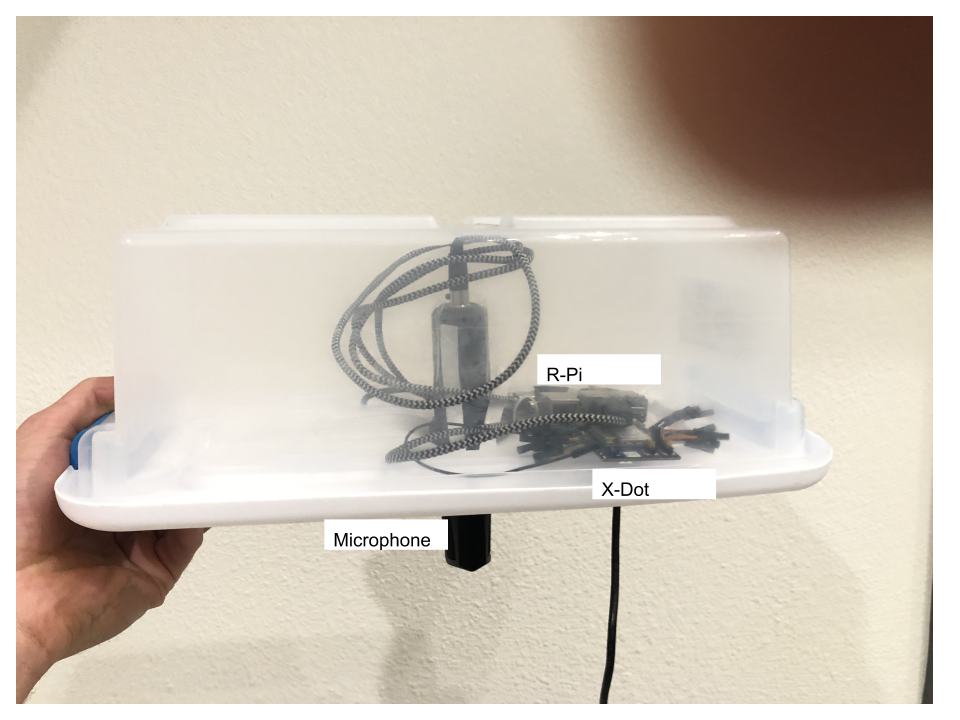
\includegraphics[width=0.7\columnwidth]{physical_system_box.png}}
\caption{Physical components assembled attached to lid of a box.}
\label{fig}
\end{figure}
\begin{figure}[htbp]
\centerline{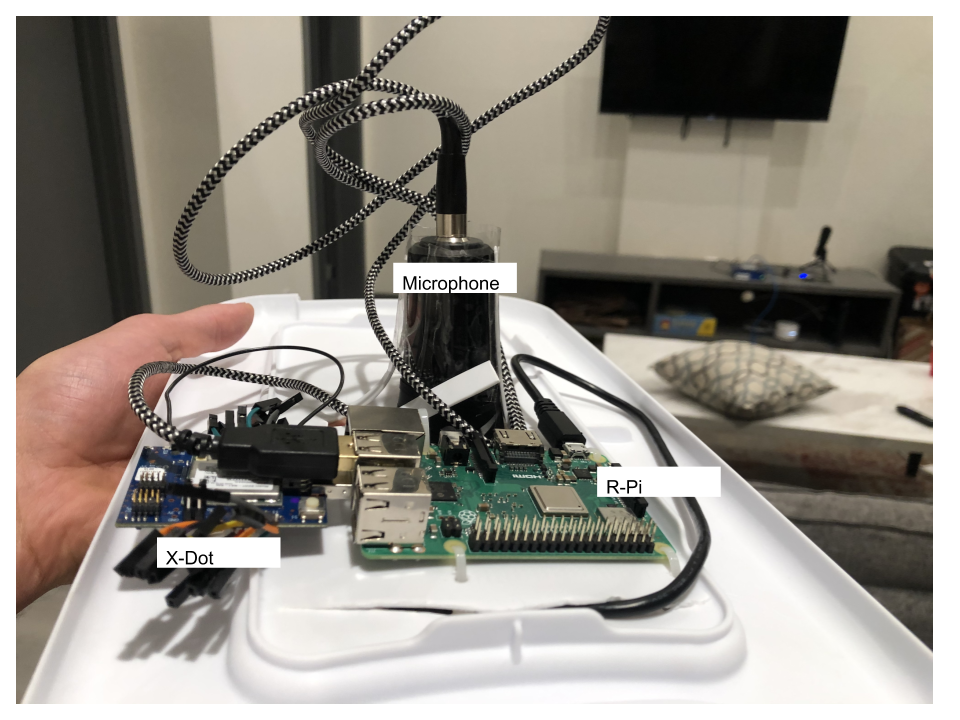
\includegraphics[width=0.7\columnwidth]{physical_system.png}}
\caption{Physical components assembled attached to lid of a box.}
\label{fig}
\end{figure}
\begin{enumerate}
\item Microphone Audio Sensor 
\item Raspberry pi
\item Multitech xDot

\end{enumerate}

The microphone is constantly recording audio and storing it in the Raspberry Pi. The Raspberry Pi will constantly check if audio amplitude exceeds a predefined threshold. This threshold was determined by analyzing audio data that could be considered noise and comparing it to gunshot audio data. 
Once the threshold is surpassed, the audio data stored in the buffer will be windowed and sent through our machine learning model which outputs the predicted sound with corresponding levels of confidence. We have made use of multithreading so that we do not miss audio data while we are running a previous window through the machine learning model.

If a gunshot was indeed heard than that information is sent to the xDot over a USB serial port. The xDot is running code that reads from its serial port, transmits the data via the sx1276 LoRa radio, and replies over the serial port when it is ready to send again. This handshake guarantees that the information about the detected gunshot is sent to the conduit.


\subsection{Network Overview}
A single network consists of several individual nodes around a multitech conduit pre-loaded with Node-Red. The conduit receives two main pieces of information from the xDots over lora radio: the confidence of a detected gunshot and the timestamp at which it was detected. By sending data over lora radio instead of another method like wifi we get two main benefits, longer range and lower costs.

 
\begin{itemize}
\item Higher Range\\  Lora signals have a range of 10 km if there is direct line of sight. 
We will be able to achieve that line of sight because our product will be placed high up out of the way of everyday life. This means that we will not need to have too many conduits to cover a very large area. 
\item Lower Costs \\ Other competing systems utilize wifi to post their data. This leads to a higher recurring costs as a SIM card is needed for each node.

\end{itemize}

On node-red the data is converted to a json object and then sent to the cloud. The only requirement to connect to the cloud is to create a HTTP request node with the URL being the endpoint from the AWS account
\section{AWS Cloud Overview}

Our project makes use of a handful of AWS applications: IoT Core, Lambda, and S3. IoT Core is an application that receives messages from IoTs and publishes those messages to an MQTT topic. Lambda is an event-driven, serverless computing platform provided by Amazon as a part of Amazon Web Services. It is a computing service that runs code in response to events and automatically manages the computing resources required by that code. S3, or Simple Storage Service, is a service offered by AWS that provides object storage through a web interface.

Data from the conduit is passed over to IoT Core. In the IoT Core all messages sent by the xDot are available in the topic in JSON format. The object contains the device’s embedded unique ID (EUI), timestamp, gun-shot confidence and the volume. However, these messages are not saved by default and need to be saved into S3. To save messages into S3, we invoke a rule, that saves a given message to S3. It is possible to save the files such that the files are named [Device EUI].json. By doing this, all messages stored in the S3 Bucket are current JSON objects and this allows us to iteratively search through the bucket. Searching through all the JSON files allows us to find the three nodes that heard the gunshots first to pinpoint the location of the gunshot.

\subsection {Multilateration}

\begin{figure}[htbp]
\centerline{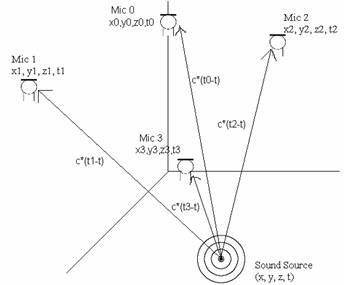
\includegraphics[width=0.7\columnwidth]{triangulate.png}}
\caption{Multilateration using audio data.}
\label{fig}
\end{figure}
To pinpoint the location of the gunshot, we need to run a function. Lambda is perfect for this because it can be set to only activate based on a trigger. The trigger is a condition that, if met, calls the function, giving us our desired output. The trigger we set is that if a gunshot message is heard on IoT Core, activate the lambda function. Our function iteratively finds the three nodes that heard it the soonest and grabs the timestamp and EUI of the nodes. The location of the nodes is saved in a lookup table referenced by the EUI. By using the EUIs, we can find the GPS location of the nodes that heard the gunshot. The GPS location is in standard WGS84 format and is then converted to Cartesian coordinates. After converting the coordinates, we run a multilateration algorithm based on Bancroft’s Algorithm \cite{b5}. This algorithm makes use of differences in Times of Arrival (TOA) of a signal and locations of base stations (our nodes) to pinpoint the location of the sender of the signal. In our case, the signal is a sound wave and the velocity of a sound wave is 343 m/s. By using this, we can accurately obtain the Cartesian coordinates of where the sound originated and convert it back to GPS coordinates.



\section{Time Synchronization}
Initially, we were going to use the built in time stamps that go along with the LoRaWAN protocol. However, we soon realized that there could be inaccuracies on the order of seconds due to where the gunshot lies in the sliding window. If by chance, the gunshot is at the start of the window on one node and the end of a window on another node, we would detect a multiple second time difference, which is incorrect. 

To fix this, we normalize the clock on the Raspberry Pi to the Master clock running on AWS. To do this, we send the Raspberry pi time almost instantaneously, and at least with equal delay at every node, to the conduit. There we calculate the time difference between that node’s time and the master time. We store this conversion factor in a lookup table, which allows for easy conversion to real time whenever we receive a Raspberry Pi time stamped message. The Raspberry Pi stamps a window with the time at which the peak sound (assumed to be the gunshot) was detected.

\section{Machine Learning Model}
We used a pretrained model called YAMNet  \cite{b6}. YAMNet is a pre-trained deep net that predicts an audio event class based on a the AudioSet-Youtube corpus (a massive collection of manually annotated audio samples). The following describes how YAMNet was trained: 
\begin{itemize}
    \item All audio is resampled to 16kHz mono
    \item A spectrogram is computed using magnitudes of Short-Time Fourier Transform with a window size of 25ms, a window hop of 10ms, and a periodic Hann window
    \item A mel spectrogram is computed by mapping the spectrogram to 64 mel bins covering the range 125-7500Hz
    \item The stabilized log mel spectrogram is computed 
  \item These features are framed with 50\% overlap. 
\end{itemize}
The following paragraph, taken from YAMNet’s README explains training the model using this extracted data:
\begin{quote}
"These patches are then fed into the Mobilenet\_v1 model to yield a 3x2 array of activations for 1024 kernels at the top of the convolution. These are averaged to give a 1024-dimension embedding, then put through a single logistic layer to get the 521 per-class output scores corresponding to the 960 ms input waveform segment."
\end{quote}


\section{Results}


\paragraph{Gunshot Detection}
In order to test our false positive we decided to use Youtube audio. The most common cause of false gunshot detection is fireworks. We played a 10 minute video of nonstop fireworks going off and our system detected gunshots BLANK TIMES.

To verify our system can detect real gunshots we visited the Los Angeles Gun Club. While there we ran our system for ten minutes and recorded the results. During those ten minutes a hundred-nineteen gunshots were fired. Our system successfully detected a hundred-thirteen of them and detected size of them as fireworks.


\begin{table}[htbp]
\caption{}
\begin{center}
 \begin{tabular}{||c || c||} 
 \hline
False Positive Rate &  \\ 
 \hline
False Negative Rate & 0.0504\\
 \hline
True Positive Rate &0.9496\\
 \hline
\end{tabular}
\label{tab1}
\end{center}
\end{table}

\paragraph{Triangulation}
We first tested the triangulation on AWS with fed data. As previously mentioned the triangulation function in Lambda is triggered when an S3 bucket is updated. Once triggered it will iterate through and pull device\_id, timestamp, lattitude, and longitude for each node. In order to test triangulation we had fixed data in the S3 lookup table for timestamp, lattitude, and longitude. The device\_ids are generated from Node-red.The values we put are reflected in table  \ref{tab1} and table  \ref{tab2}.



\begin{table}[htbp]
\caption{Each device has a unique ID and a detection timestamp }
\begin{center}
 \begin{tabular}{||c | c||} 
 \hline
device\_id & timestamp \\ [0.5ex] 
 \hline\hline
 00-80-00-00-04-01-76-64 & 12:24:49 \\ 
 \hline
 00-80-00-00-04-01-76-2B & 12:24:51 \\
 \hline
 00-80-00-00-04-01-75-EC & 12:24:52\\
 \hline
\end{tabular}
\label{tab1}
\end{center}
\end{table}
\begin{table}[htbp]
\caption{Latitude and Longitude of each node are stored in a look up table }
\begin{center}
 \begin{tabular}{||c |c  c||} 
 \hline
&Latitude & Longitude \\ [0.5ex] 
 \hline\hline
Node 1 & 34.025277 & -118.291241 \\ 
 \hline
Node 2 & 34.018477 & -118.291364\\
 \hline
Node 3 & 34.020545 & -118.285404\\
 \hline
\end{tabular}
\label{tab2}
\end{center}
\end{table}

The artificial coordinates of Node 1, Node 2, and Node 3 are placed on the University of Southern California campus represent Jefferson \& Vermont, Expo \& Vermont, and Tommy Trojan respectively.

\begin{figure}[htbp]
\centerline{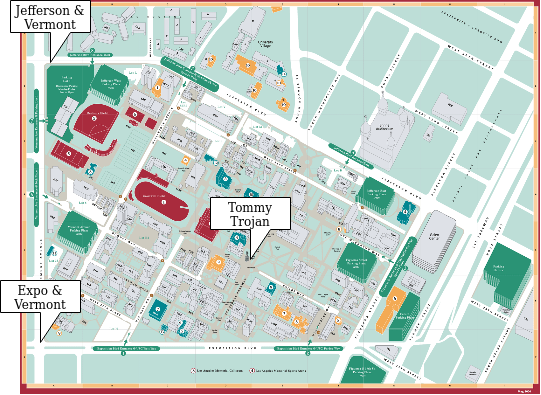
\includegraphics[width=0.9\columnwidth]{nodes_usc.png}}
\caption{Visualization of node placement}
\label{fig}
\end{figure}

Our Lambda function successfully pulled in the  correct id's and coordinates. From there it used the gunshot detection timestamps to generate gps coordinates of the likely gunshot location. With this input data our function generates the following:


\begin{small}
\begin{verbatim}
{
  "statusCode": 100,
  "body": "\"where the gunshot occurred\"",
  "lat": "34.022294",
  "long": "-118.289687"
}
\end{verbatim}
\end{small}

When the coordinates are plotted we see that it is very close to the center of the three nodes which makes logical sense. The location is not perfect because minute changes in latitude and longitude map into a significant distance difference.

%
%\begin{center}
%\begin{tabular}{ c c c }
% cell1 & cell2 & cell3 \\ 
%\hline
% cell4 & cell5 & cell6 \\  
%\hline
% cell7 & cell8 & cell9    
%\end{tabular}
%\end{center}




%\begin{tabularx}{0.8\textwidth} { 
%  | >{\raggedright\arraybackslash}X 
%  | >{\centering\arraybackslash}X 
%  | >{\raggedleft\arraybackslash}X | }
% \hline
% item 11 & item 12 \\
% \hline
% item 21  & item 22\\
%\hline
%\end{tabularx}





%\begin{table}[htbp]
%\caption{Table Type Styles}
%\begin{center}
%\begin{tabular}{|c|c|c|c|}
%\hline
%\textbf{Table}&\multicolumn{3}{|c|}{\textbf{Table Column Head}} \\
%\cline{2-4} 
%\textbf{Head} & \textbf{\textit{Table column subhead}}& \textbf{\textit{Subhead}}& \textbf{\textit{Subhead}} \\
%\hline
%copy& More table copy$^{\mathrm{a}}$& &  \\
%\hline
%\multicolumn{4}{l}{$^{\mathrm{a}}$Sample of a Table footnote.}
%\end{tabular}
%\label{tab1}
%\end{center}
%\end{table}



\section*{Acknowledgment}

We would like to acknowledge our Internet and Cloud Computiong Professor, Dr. Young Cho and our Internet and Cloud Computing  Teaching Assistant Arthur Win.


\begin{thebibliography}{00}
\bibitem{b1} Centers for Disease Control and Prevention, The Steady Rise Of U.S. Gun Deaths. statista.
\bibitem{b2} L. G. Mazerolle, “Using gunshot detection technology in high-crime areas,” in Using gunshot detection technology in high-crime areas, 1998.


\bibitem{b3} B. Fraga, “After Too Many Shots Missed, Fall River, Mass., Ends Deal with ShotSpotter,” Government Technology State \& Local Articles - e.Republic. [Online]. Available: https://www.govtech.com/public-safety/After-Too-Many-Shots-Missed-Fall-River-Mass-Ends-Deal-with-ShotSpotter.html. [Accessed: 13-Dec-2019].
\bibitem{b4}ShotSpotter, “PRICE PROPOSAL FOR SUBSCRIPTION-BASED SHOTSPOTTER®GUNFIRE LOCATION, ALERT AND ANALYSIS SERVICE FOR THE CITY OF DURHAM,” cityordinances.durhamnc.gov. [Online]. Available: https://cityordinances.durhamnc.gov/OnBaseAgendaOnline/Documents/
ViewDocument/WS-Published Attachment - 13024 - PROPOSAL - 2 SPOTSHOTTER FOR DURHAM - 3\_18.pdf?meetingId=296\&documentType=Agenda\&itemId=10442\&pub
lishId=47466\&isSection=false.
\bibitem{b5} M. Geyer and A. Daskalakis, “Solving passive multilateration equations using Bancrofts algorithm,” 17th DASC. AIAA/IEEE/SAE. Digital Avionics Systems Conference. Proceedings (Cat. No.98CH36267).
\bibitem{b6} D. Ellis and M. Plakal, "YAMNet", GitHub repository, Available: https://github.com/tensorflow/models/tree/master/research/audioset/yamnet

\end{thebibliography}

\end{document}